\documentclass[crop,tikz]{standalone}

% Field lines of an electric field inside and outside of a polarized
% sphere of radius R inside an infinitely large plate capacitor.
%
% The potential is independent of \varphi and is thus given by
%
% \phi(r,\theta) = -Ar\cos(\theta) + B\cos(\theta)/r^2,

% where A,B are given by the boundary conditions on the sphere:
% A=(\epsilon_r+2)/3E_i, B=(\epsilon_r-1)/3E_iR^3, where E_i is the
% field strength inside the sphere. So, the components of the electric
% field are
%
% E_r(r,\theta) = E_i\cos(\theta)[(\epsilon_r+2)/3+2(\epsilon_r)R^3/r^3/3],
% E_\theta(r,\theta) = -E_i\sin(\theta)[(\epsilon_r+2)/3-(\epsilon_r-1)R^3/r^3/3],
% E_z(r,\theta) = E_r(r,\theta)\cos(\theta)-E_\theta(r,\theta)\sin(\theta),
% E_y(r,\theta) = E_r(r,\theta)\sin(\theta)+E_\theta(r,\theta)\cos(\theta).
% 
% A field line is tangential to the electric field, so
%
% dr/d\theta = rE_r/E_\theta .

% Inserting E_r and E_\theta and solving the differential equation
% yields the condition
%
% (E_0r^3+3B)\sin^2(\theta) = b^2r

% where E_0=E_i(\epsilon_r+2)/3 and B=-E_i(\epsilon_r-1)R^3 and b is
% an arbitrary constant. Solving yields
%
% \sin^2(\theta(r)) = b^2r/(r^3+2B/E_0) .

% We chose t := r (>= R) as parameter. The parametrization can then be
% expressd by a function \rho(t)=x(t), which describes the distance
% from the z axis and z(t) with
%
% \rho(t) = t\sin(\theta(t)) = b\sqrt{t^3/(t^3+2B/E_0)},
% z(t) = t\sin(\theta(t)) = \pm\sqrt{t^2-\rho^2(t)}.

\usetikzlibrary{decorations.markings}

\tikzset{%
  >=latex, % default arrow style
  ->-/.style={postaction={decorate},decoration={%
      markings,mark=at position #1 with {\arrow{>}}%
    }%
  },%
  ->-/.default=.5,%
  -<-/.style={postaction={decorate},decoration={%
      markings,mark=at position #1 with {\arrowreversed{>}}%
    }%
  },%
  -<-/.default=.5%
}

\usepackage{pgfplots}
\pgfplotsset{compat=1.13}

\pgfplotsset{
  inverted/.style = {
    every axis legend/.append style={
      draw=white,
      fill=hardblack,
      text=white
    }
  },
}

\begin{document}
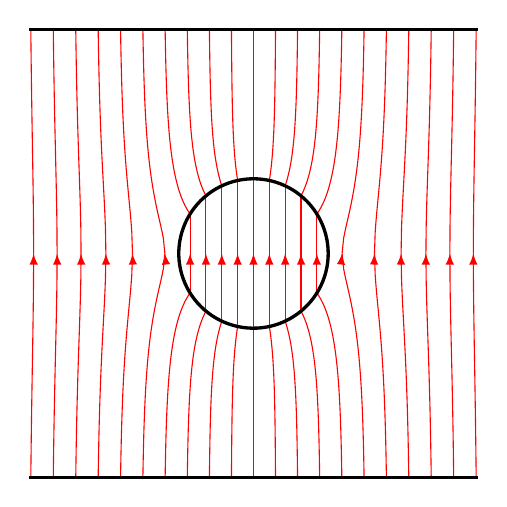
\begin{tikzpicture}
  \pgfmathsetmacro{\tmax}{5} % maximum parameter value
  \pgfmathsetmacro{\xmax}{3} % size of plot
  \pgfmathsetmacro{\R}{1.0} % radius of sphere
  \pgfmathsetmacro{\epsr}{4.0} % dielectric constant
  \pgfmathsetmacro{\Ei}{1.0} % field strength inside sphere
  \pgfmathsetmacro{\k}{2*(\epsr-1)/(\epsr+2)}
  \pgfmathsetmacro{\bmin}{0} % minimum value for b
  \pgfmathsetmacro{\btouch}{sqrt(1+\k)} % maximum value for b so that field lines touch sphere
  \pgfmathsetmacro{\bmax}{\xmax/\R} % maximum reasonable value for plot size
  \pgfmathsetmacro{\Nb}{11} % number of fieldlines
  \pgfmathtruncatemacro{\NbmOne}{\Nb-1}
  \pgfmathsetmacro{\db}{(\bmax-\bmin)/\NbmOne} % step size for b
  \begin{axis}[
    view={0}{90},
    axis equal image,
    xmin={-\xmax}, xmax={\xmax},
    ymin={-\xmax}, ymax={\xmax},
    hide axis,
    clip=false,
    unbounded coords=discard,
    samples=100,
    xlabel={$x$},
    ylabel={$y$},
    declare function={
      rhoOverR(\t,\b) = \b*sqrt(\t^3/(\t^3 + \k)); % \rho(t)/R
      zOverR(\t,\b)   = sqrt(max(0, \t^2 - rhoOverR(\t,\b)^2)); % z(t)/R
      % turning point for t: largest positive solution of t^3 - b^2 t + k = 0
      argturn(\b) = max(-1, min(1,-3*sqrt(3)*\k/(2*\b^3)));
      tturn(\b) = 2*\b/sqrt(3)*cos(acos(argturn(\b))/3);
      % rr(\x,\y) = sqrt(\x*\x + \y*\y);
      % theta(\x,\y) = atan2(\y,\x);
      % Er(\x,\y) = \Ei*cos(theta(\x,\y))*((\epsr+2)/3 + 2/3*(\epsr-1)*\R^3/(rr(\x,\y)^3));
      % Etheta(\x,\y) = -\Ei*sin(theta(\x,\y))*((\epsr+2)/3 - (\epsr-1)/3*\R^3/(rr(\x,\y)^3));
      % Ez(\x,\y) = Er(\x,\y)*cos(theta(\x,\y)) - Etheta(\x,\y)*sin(theta(\x,\y));
      % Ey(\x,\y) = Er(\x,\y)*sin(theta(\x,\y)) + Etheta(\x,\y)*cos(theta(\x,\y));
      % Ea(\x,\y) = sqrt(Ez(\x,\y)^2 + Ey(\x,\y)^2);
    },
    ]
    % \addplot3[
    %   red,
    %   -Stealth,
    %   quiver={
    %     u={ifthenelse(rr(x,y)<\R, 0, Ey(x,y)/Ea(x,y))},
    %     v={ifthenelse(rr(x,y)<\R, 1, Ez(x,y)/Ea(x,y))},
    %     scale arrows=0.3,
    %   },
    %   domain=-3:3,
    %   domain y=-3:{3-2/15-0.3},
    %   samples=15,
    %   samples y=15,
    % ] ({x},{y},{0});
    \begin{scope}
      \clip ({-\xmax},{-\xmax}) rectangle ({\xmax},{\xmax});
      % fieldline for \rho=0
      \addplot[red,thin,->-] coordinates {(0,-\R*\tmax) (0,\R*\tmax)};
      % fieldlines for \rho>0
      \pgfplotsinvokeforeach{1,...,\NbmOne}{%
        \pgfmathsetmacro{\b}{\bmin + (#1)*\db}
        \pgfmathsetmacro{\rhozero}{rhoOverR(1,\b)} % rho0/R
        \pgfmathtruncatemacro{\hit}{ifthenelse(\rhozero<=1,1,0)} % field line touches sphere?
        \ifnum\hit=1
          % outside sphere
          \addplot[red,thin,domain=1:{\tmax}] ({ \R*rhoOverR(x,\b)}, { \R*zOverR(x,\b)});
          \addplot[red,thin,domain=1:{\tmax}] ({ \R*rhoOverR(x,\b)}, {-\R*zOverR(x,\b)});
          \addplot[red,thin,domain=1:{\tmax}] ({-\R*rhoOverR(x,\b)}, { \R*zOverR(x,\b)});
          \addplot[red,thin,domain=1:{\tmax}] ({-\R*rhoOverR(x,\b)}, {-\R*zOverR(x,\b)});
          % inside sphere
          \pgfmathsetmacro{\zmax}{sqrt(1 - \rhozero^2)} % z/R
          \addplot[red,thin,->-] coordinates { ( \R*\rhozero, -\R*\zmax) ( \R*\rhozero, \R*\zmax) };
          \addplot[red,thin,->-] coordinates { (-\R*\rhozero, -\R*\zmax) (-\R*\rhozero, \R*\zmax) };
        \else
          \pgfmathsetmacro{\tmin}{max(1, tturn(\b))}
          \addplot[red,thin,domain=\tmin:\tmax,->-=0] ({ \R*rhoOverR(x,\b)}, { \R*zOverR(x,\b)});
          \addplot[red,thin,domain=\tmin:\tmax] ({ \R*rhoOverR(x,\b)}, {-\R*zOverR(x,\b)});
          \addplot[red,thin,domain=\tmin:\tmax,->-=0] ({-\R*rhoOverR(x,\b)}, { \R*zOverR(x,\b)});
          \addplot[red,thin,domain=\tmin:\tmax] ({-\R*rhoOverR(x,\b)}, {-\R*zOverR(x,\b)});
        \fi
      }
    \end{scope}
    % sphere
    \addplot[black,very thick,domain=0:360,samples=100] ({\R*cos(x)}, {\R*sin(x)});
    % capacitor
    \draw[very thick] ({-\xmax},{\xmax}) -- ({\xmax},{\xmax});
    \draw[very thick] ({-\xmax},{-\xmax}) -- ({\xmax},{-\xmax});
  \end{axis}
\end{tikzpicture}
\end{document}
